% !TEX program = xelatex
% 공통수학2 · Ⅰ. 도형의 방정식 · 3. 도형의 이동 · 02 대칭이동 · 1/2차시
% 학생용 활동지 (답안 없음)
\documentclass[11pt,a4paper]{article}
\usepackage{kotex}
\usepackage{iftex}
\ifPDFTeX\else
  \setmainhangulfont{Noto Serif CJK KR}
  \setsanshangulfont{Noto Sans CJK KR}
\fi
\usepackage[margin=2.1cm]{geometry}
\usepackage{parskip}
\usepackage{enumitem}
\usepackage{array}
\usepackage{tabularx}
\usepackage{xcolor}
\usepackage{amssymb}
\usepackage{tikz}
\usepackage[most]{tcolorbox}
\usepackage{fancyhdr}
\usepackage{titlesec}

\definecolor{goldc}{HTML}{B07C22}
\definecolor{goldstrong}{HTML}{8A5F16}
\definecolor{indigoc}{HTML}{2B3B57}
\definecolor{indigosoft}{HTML}{6E82A6}
\definecolor{linec}{HTML}{D6DACB}
\definecolor{surface2}{HTML}{E4E8DC}
\definecolor{writeline}{HTML}{C7CCBA}
\definecolor{inksoft}{HTML}{52604F}

\titleformat{\section}{\normalfont\sffamily\bfseries\large\color{indigoc}}{\thesection}{0.6em}{}
\titlespacing{\section}{0pt}{14pt}{6pt}
\newtcolorbox{goalbox}{enhanced, breakable, colback=white, colframe=goldc, boxrule=0.5pt, leftrule=3pt, arc=2pt, left=10pt, right=10pt, top=8pt, bottom=8pt}
\newtcolorbox{sheetbox}{enhanced, breakable, colback=white, colframe=linec, boxrule=0.6pt, arc=3pt, left=11pt, right=11pt, top=9pt, bottom=9pt}
\newcommand{\writespace}[1]{%
  \par\nobreak\vspace{3pt}
  \foreach \n in {1,...,#1} {%
    \noindent\textcolor{writeline}{\rule{\linewidth}{0.4pt}}\par\vspace{0.62cm}%
  }
}
\newcommand{\fillblank}[1]{\makebox[#1]{\hrulefill}}
\pagestyle{fancy}\fancyhf{}\renewcommand{\headrulewidth}{0pt}
\fancyfoot[L]{\footnotesize\color{inksoft} 공통수학2 · 2026학년도 2학기 · 지평선고등학교}
\fancyfoot[R]{\footnotesize\color{inksoft} 다음 시간 --- 02 대칭이동(2) 도형의 대칭이동}

\begin{document}

\noindent
\begin{minipage}[b]{0.62\linewidth}
  {\sffamily\footnotesize\color{indigosoft} 공통수학2 · Ⅰ. 도형의 방정식 · 3. 도형의 이동}\\[2pt]
  {\sffamily\bfseries\Large 02 대칭이동 \textperiodcentered\ 15차시}
\end{minipage}\hfill
\begin{minipage}[b]{0.36\linewidth}
  \raggedleft\small\color{inksoft}
  반\ \fillblank{1.6cm} \quad 번호\ \fillblank{1.6cm}\\[4pt]
  이름\ \fillblank{3.6cm}
\end{minipage}

\vspace{4pt}
\noindent{\color{goldc}\rule{\linewidth}{2.2pt}}
\vspace{10pt}

\begin{goalbox}
\textbf{오늘의 목표}\\
점을 $x$축, $y$축, 원점, 직선 $y=x$에 대하여 대칭이동한 점의 좌표를 구할 수 있다.
\vspace{4pt}
\small\color{inksoft}
$\square$ 자신 있음 \quad $\square$ 조금 헷갈림 \quad $\square$ 처음 봄 \hfill (수업 전 나의 상태에 표시)
\end{goalbox}

\section{생각 열기 --- 만자창 무늬}

\begin{sheetbox}
아래는 만자창 무늬를 좌표평면 위에 나타낸 것이다. 점 A$(1,2)$가 있을 때, $x$축에 대하여 대칭인 점을 B, $y$축에 대하여 대칭인 점을 C, 원점에 대하여 대칭인 점을 D라 하자.

\begin{center}
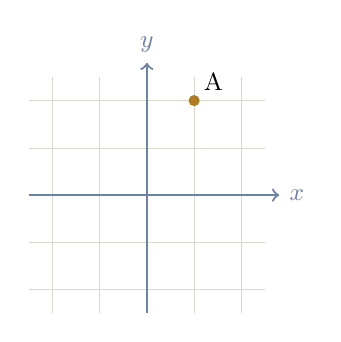
\begin{tikzpicture}[scale=0.6]
  \draw[step=1cm, linec, very thin] (-2.5,-2.5) grid (2.5,2.5);
  \draw[->, thick, indigosoft] (-2.5,0) -- (2.8,0) node[right, font=\small]{$x$};
  \draw[->, thick, indigosoft] (0,-2.5) -- (0,2.8) node[above, font=\small]{$y$};
  \filldraw[goldc] (1,2) circle (3pt);
  \node[above right, font=\small] at (1,2) {A};
\end{tikzpicture}
\end{center}

\begin{enumerate}[leftmargin=1.4em, itemsep=2pt]
  \item 위 그림에 점 B, C, D를 직접 표시해 보자.
  \item 점 A, B, C, D의 좌표를 각각 말해 보자.
\end{enumerate}
\writespace{3}
\end{sheetbox}

\section{개념 정리 --- 점의 대칭이동}

\begin{sheetbox}
점 $(x,y)$를
\begin{enumerate}[leftmargin=1.6em, itemsep=3pt]
  \item $x$축에 대하여 대칭이동한 점의 좌표는 $\left(\ \fillblank{2cm}\ ,\ \ \fillblank{2cm}\ \right)$
  \item $y$축에 대하여 대칭이동한 점의 좌표는 $\left(\ \fillblank{2cm}\ ,\ \ \fillblank{2cm}\ \right)$
  \item 원점에 대하여 대칭이동한 점의 좌표는 $\left(\ \fillblank{2cm}\ ,\ \ \fillblank{2cm}\ \right)$
  \item 직선 $y=x$에 대하여 대칭이동한 점의 좌표는 $\left(\ \fillblank{2cm}\ ,\ \ \fillblank{2cm}\ \right)$
\end{enumerate}

\vspace{8pt}
\textbf{생각해보기} --- 직선 $y=-x$에 대하여 대칭이동한 점 $(x,y)$의 좌표는 무엇일까? (힌트: 중점이 $y=-x$ 위에 있고, PP$'\perp y=-x$)
\writespace{3}
\end{sheetbox}

\section{연습 문제}

\begin{sheetbox}
\textbf{1.} 점 $(3,-5)$를 다음에 대하여 대칭이동한 점의 좌표를 구하시오.\\
\hspace*{1.6em}⑴ $x$축 \quad ⑵ $y$축 \quad ⑶ 원점 \quad ⑷ 직선 $y=x$
\writespace{4}
\end{sheetbox}

\section{사고의 가시화 --- See · Think · Wonder}

\noindent{\footnotesize\color{inksoft} 오늘 배운 `대칭이동'을 떠올리며 아래 세 칸을 채워 보자.}\\[6pt]
\begin{tabularx}{\linewidth}{@{}XXX@{}}
\textbf{\footnotesize\color{indigoc} See --- 무엇을 보았나?} &
\textbf{\footnotesize\color{indigoc} Think --- 무엇을 생각했나?} &
\textbf{\footnotesize\color{indigoc} Wonder --- 무엇이 궁금한가?} \\[4pt]
\end{tabularx}
\noindent
\begin{minipage}[t]{0.32\linewidth}\writespace{3}\end{minipage}\hfill
\begin{minipage}[t]{0.32\linewidth}\writespace{3}\end{minipage}\hfill
\begin{minipage}[t]{0.32\linewidth}\writespace{3}\end{minipage}

\section{마무리 성찰}

\begin{sheetbox}
\begin{minipage}[t]{0.48\linewidth}
{\footnotesize\color{inksoft} 오늘 배운 것을 한 문장으로}
\writespace{2}
\end{minipage}\hfill
\begin{minipage}[t]{0.48\linewidth}
{\footnotesize\color{inksoft} 감사 일기 / 유념 한 줄}
\writespace{2}
\end{minipage}
\end{sheetbox}

\end{document}
